\section*{Vehicle Models and Simulations}

\begin{frame}{Vehicle Models}
    \textbf{Point Mass:}
    Vehicle is treated as a concentrated point mass.
    Useful for analysing basic sensitivities.
    \\~\\
    \textbf{Bicycle Model:}
    Vehicle is represented by a front and rear axle.
    Longitudinal load transfer occurs when braking and accelerating.
    \\~\\
    \textbf{Four Corner:}
    All four tyres of the vehicle are represented.
    Both lateral and longitudinal load transfer are considered.
    \\~\\
    \textbf{Four Corner with Suspension:}
    Effects of suspension geometry (camber, toe, etc.) are considered.
    Useful for optimising vehicle setup.
\end{frame}

\begin{frame}{Simulation Types}
    \textbf{Quasi-Steady-State (QSS) Simulation:}
    Acceleration is constant in each section of the track mesh.
    Simple to solve, but unable to account for transient effects
    such as yaw acceleration or cell temperatures.
    \\~\\
    \textbf{Transient Simulation:}
    Transient effects like temperature are modelled.
    Much more complicated to solve than QSS,
    but able to explore more complex vehicle behaviour.
    \\~\\
    \textbf{Driver-in-the-Loop (DITL) Simulation:}
    The vehicle is simulated in real-time,
    with control inputs provided by the driver.
    Able to explore the `driveability' of a vehicle,
    but also subject to driver error. 
\end{frame}

\begin{frame}{Time vs Distance Basis}
    \begin{columns}
        \column{0.5\textwidth}
        \hfill \textbf{Time Basis} \hfill
        \begin{itemize}
            \item Each step takes a fixed amount of time
            \item Distance calculated with $s = ut + \frac{1}{2}at^2$
            \item Good at simulating the acceleration event
        \end{itemize}
        \column{0.5\textwidth}
        \hfill \textbf{Distance Basis} \hfill
        \begin{itemize}
            \item Each step is a fixed distance
            \item Time calculated with $t = s / v_\text{avg}$
            \item Good at simulating autocross and endurance events
        \end{itemize}
    \end{columns}
    \begin{columns}
        \column{0.4\textwidth}
        We can use numerical integration methods
        like the trapezoidal or the midpoint rule
        to improve accuracy.
        \column{0.3\textwidth}
        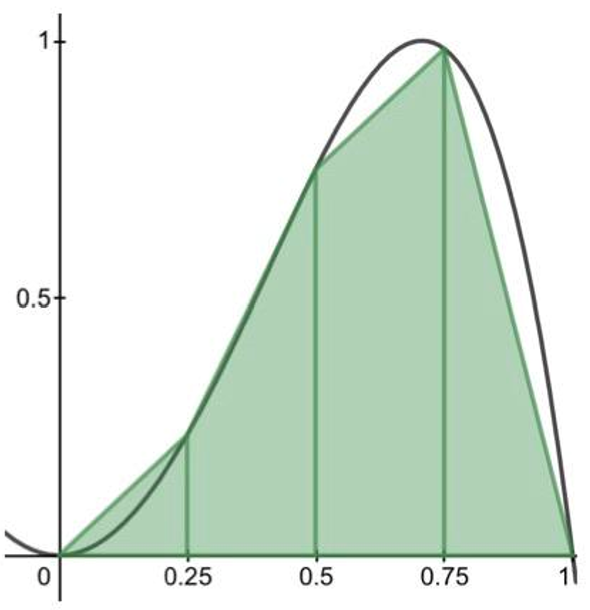
\includegraphics[width=\textwidth]{res/Trapezoidal Rule.png}
        \column{0.3\textwidth}
        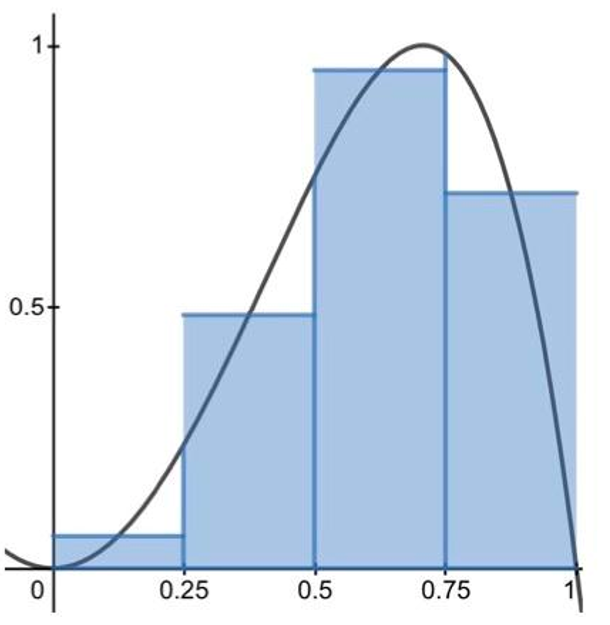
\includegraphics[width=\textwidth]{res/Midpoint Rule.png}
    \end{columns}
\end{frame}

\begin{frame}{Existing Laptime Simulations}
    \textbf{OpenLAP:}
    Open-source point mass laptime simulation written in MATLAB\@.
    Useful starting point, but vehicle model is very limited.
    \\~\\
    \textbf{Bailey and Murray's Lapsim:}
    Four corner laptime simulation written in MATLAB\@.
    Much better vehicle model
    with suspension geometry and an electric powertrain,
    and with a more accurate tyre model.
    \\~\\
    \textbf{USMLap:}
    Laptime simulation written in Python.
    Using Murray's lapsim as a starting point,
    optimised to allow it to run much faster.
    Will include a transient solver,
    allowing for accumulator state-of-charge
    and cell temperatures
    to be accounted for.
\end{frame}
